% !TeX root = probability.tex

%%%%%%%%%%%%%%%%%%%%%%%%%%%%%%%%%%%%%%%%%%%%%%%%%%%%%%%%%%%%%

\section{קיץ תשע"ח מועד ב}

\begin{center}
\selectlanguage{english}
\hspace*{8em}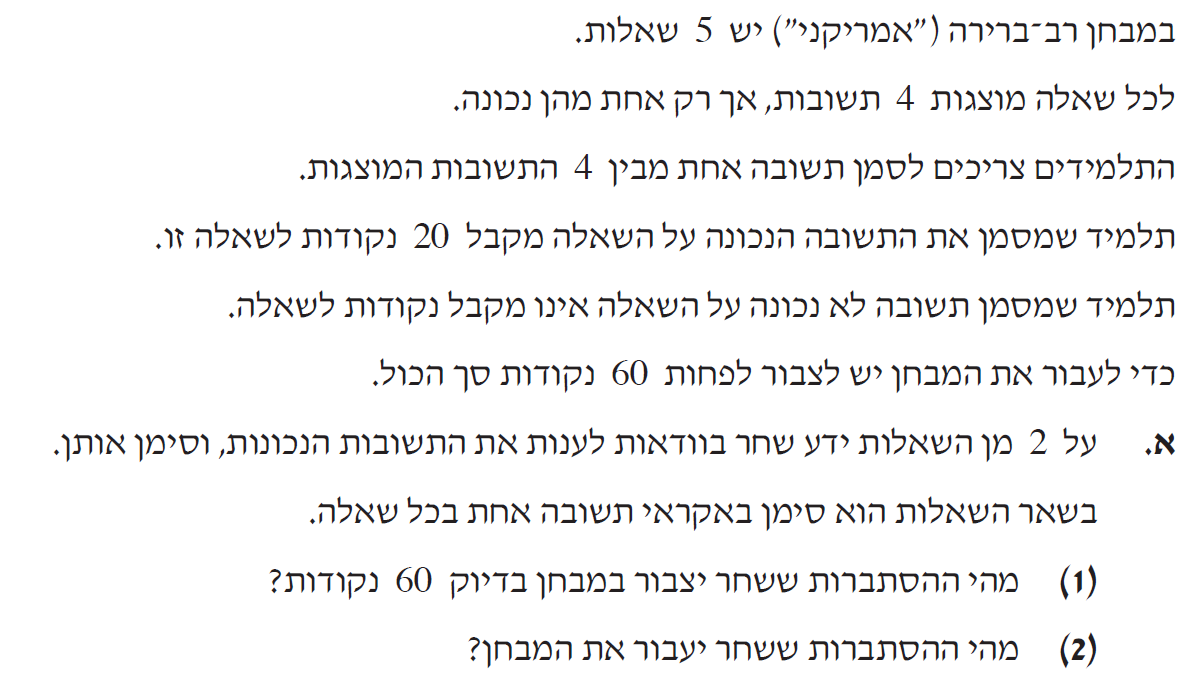
\includegraphics[width=.7\textwidth]{summer-2018b-3a}
\hspace*{-2.2em}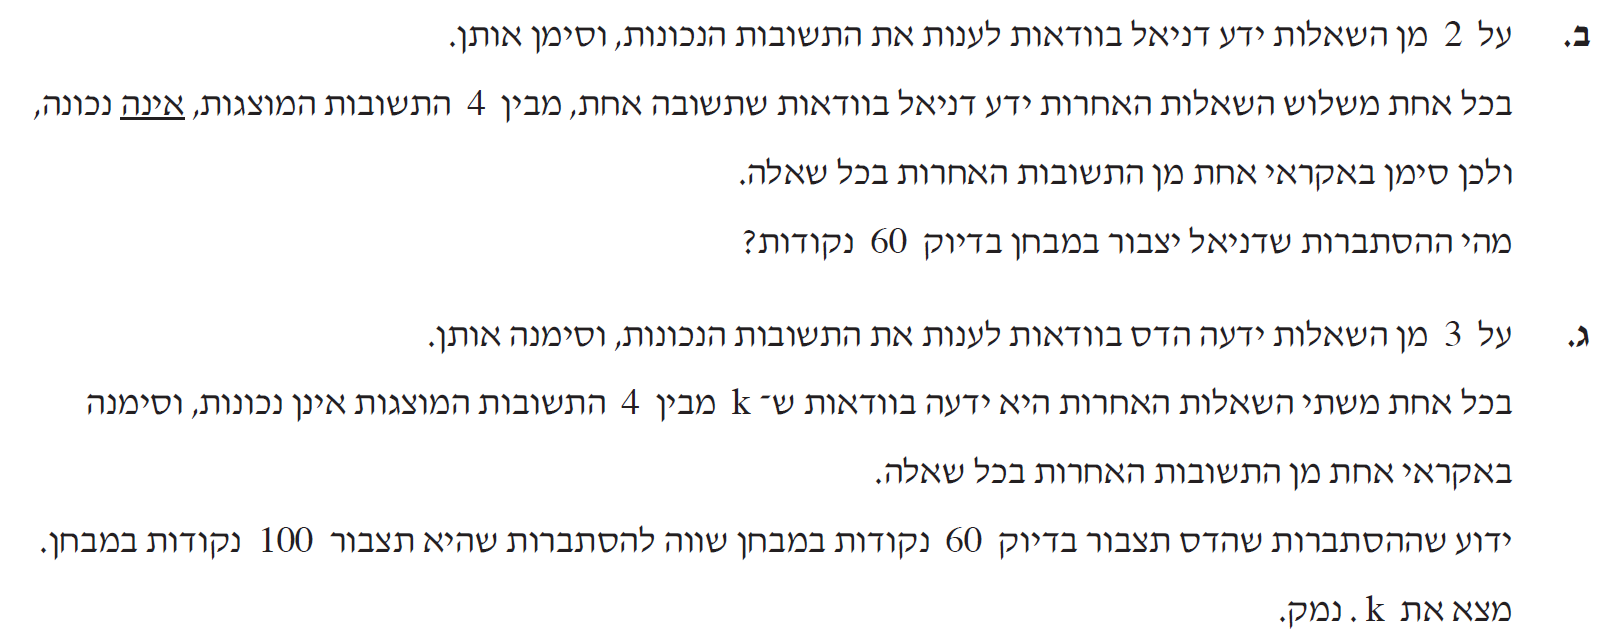
\includegraphics[width=\textwidth]{summer-2018b-3b}
\end{center}

המאורועות הם מספר הנקודות הצברות על ידי התלמידים.

השאלה מתארת הצלחות וכשלונות במתן לתשובות על המבחן ושואלת על מספר ההצלחות והכשלונות. לכן הפתרון ישתמשמ בנוסחת ברנולי.

\textbf{סעיף א}

1. שחר ידע שהוא ענה נכון על שתי שאלות ולכן כדי לקבל ציון
$60$
עליו לענות על בדיוק אחת משלושת השאלות האחרות. ההסתברות לענות נכון על שאלה היא 
$\frac{1}{4}$
ולפי נוסחת ברנולי:
\[
{3 \choose 1}\left(\frac{1}{4}\right)\left(\frac{3}{4}\right)^2=\frac{27}{64}\,.
\]
2. כדי לעבור את המבחן עליו לצבור לפחות שלוש תשובות נכונות. להסתברות מהסעיף הקודם יש להוסיף את ההסתברויות של ארבע וחמש תשובות נכונות:
\[
\frac{27}{64}+{3 \choose 2}\left(\frac{1}{4}\right)^2\left(\frac{3}{4}\right)^1+{3 \choose 3}\left(\frac{1}{4}\right)^3\left(\frac{3}{4}\right)^0=\frac{37}{64}\,.
\]

\newpage

\textbf{סעיף ב}

דניאל צריך לענות נכון על שאלה אחת בדיוק מתוך שלושת השאלות הנותרות. דניאל ידע שתשובה אחת לא נכונה, לכן ההסתברות שהוא ענה נכון על השאלה היא
$\frac{1}{3}$
ולא 
$\frac{1}{4}$
כמו בסעיף הקודם:
\[
{3 \choose 1}\left(\frac{1}{3}\right)\left(\frac{2}{3}\right)^2=\frac{4}{9}\,.
\]
\textbf{סעיף ג}

תהי
$p_k$
ההסתברות שהדס ידעה וודאות ש-%
$k$
מתוך 
$4$
תשובות לא נכונות. ההסתברות שהיא שהיא צריכה לבחור תשובה באופן אקראי היא המשלים
$1-p_k$.
כדי לקבל ציון
$60$
היא צריכה לענות נכון על אפס מתוך שתי השאלות הנוספות וכדי לקבל ציון 
$100$
היא צריכה לענות נכון על כל השאלות הנכונות. נשווה את שתי ההסתברויות המתקבלות מנוסחת ברנולי:
\begin{eqn}
{2 \choose 0}p_k^0(1-p_k)^2 &=& {2 \choose 2}p_k^2(1-p_k)^0\\
(1-p_k)^2 &=& p_k^2\\
p_k&=&\frac{1}{2}\,,
\end{eqn}
כאשר השתמשנו ב-%
${n\choose 0}={n\choose n}=1$
ו-%
$p^0=(1-p)^0=1$.

 ההסתברות שהיא ענתה תשובה נכונה לשאלה אחת היא
$p_k=\displaystyle\frac{1}{4-k}$
ולכן 
$k=2$.

\textbf{פתרון שני}

אם לא היינו מגדירים את הסימון
$p_k$
היינו מקבלים מפישוט השוויון של נוסחאות ברנולי:
\[
\left(\frac{1}{4-k}\right)^2 =\left(1-\frac{1}{4-k}\right)^2=\left(\frac{3-k}{4-k}\right)^2\,.
\]
נכפיל את שני הצדדים של המשוואה ב-%
$(4-k)^2$
ונקבל את המשוואה ריבועית
$k^2-6k+8=0$
שפתרונותיה הם 
$k=2,k=4$.
הפרמטר
$k$
מוגדר כמספר התשובות שהדס יודעת שהן אינן נכונות, ונתון שתשובה אחת נכונה, כך שיש לפסול את הפתרון
$k=4$
ולבחור
$k=2$.

האפשרות השנייה היא לקחת שורש של שני הצדדים ונקבל שתי משוואות:
\begin{eqn}
\frac{1}{4-k}&=&+\frac{3-k}{4-k}\\
\frac{1}{4-k}&=&-\frac{3-k}{4-k}\,.
\end{eqn}
מהמשוואה הראשונה נקבל
$k=2$.
מהמנה של המשוואה השנייה נקבל 
$k=4$
ונפסול אותו כי הוא מאפס את המכנה.

כל הפתרונות מגיעים לתשובה הנכונה אבל בחירה נכונה של סימון וסדר החישובים יכולים להשפוע על פשטות הפתרון.

%%%%%%%%%%%%%%%%%%%%%%%%%%%%%%%%%%%%%%%%%%%%%%%%%%%%%%%%%%%%%%

\newpage

\section{קיץ תשע"ח מועד א}

\begin{center}
\selectlanguage{english}
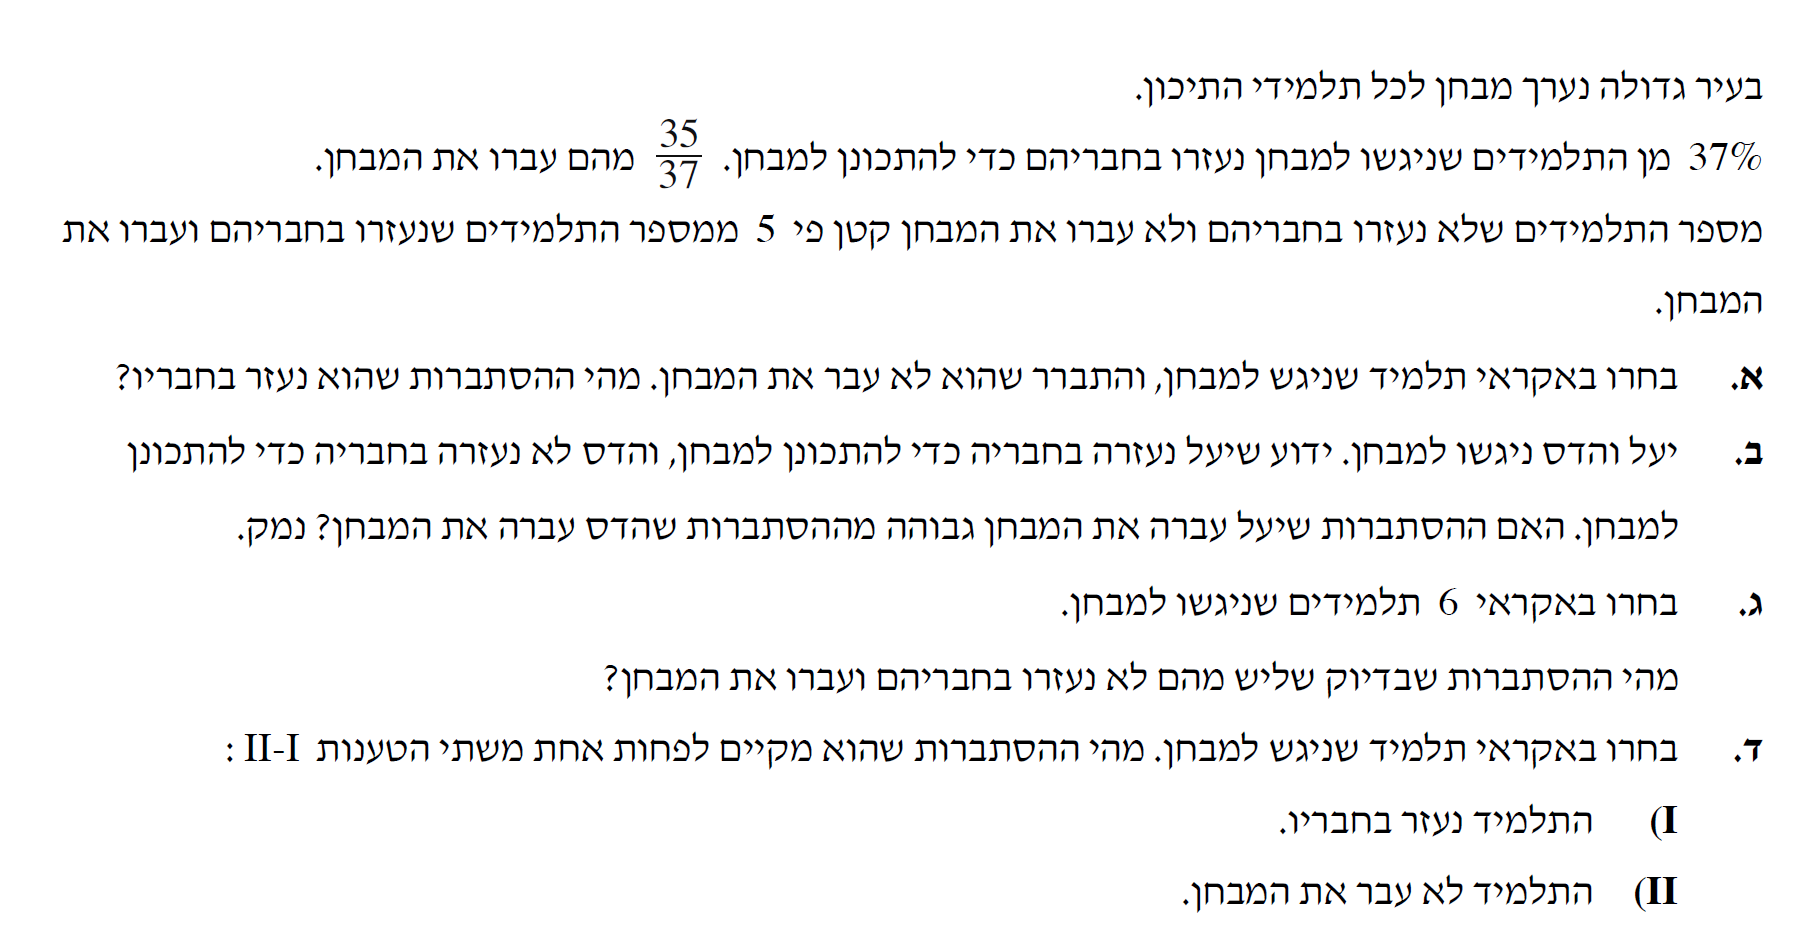
\includegraphics[width=	\textwidth]{summer-2018a-3}
\end{center}

מצאתי שניסוח השאלה מבלבל. כאשר כתוב ש-%
$37\%$
מן התלמידים ניגשו למבחן, הנטייה היא לפרש את זה כ-%
$37$
מתוך
$100$
תלמידים, כאשר אחוז למעשה מבטא יחס:
\[
37\% = \frac{37}{100} = \frac{74}{200} = \frac{18.5}{50} = \cdots\,.
\]
המשפט הבא קובע ש-%
$\frac{35}{37}$
"מהם" עברו את המבחן ואפשר לחשוב שמדובר ב-%
$35$
מתוך
$37$
תלמידים, אולם שוב מדובר ביחס. בשני המקרים יחס הוא הסתברות.

נסמן ב-%
$N$ 
\L{(ne-ezru)}
את התלמידים שנעזרו בחבריהם, וב-%
$A$
\L{(avru)}
את התלמידים שעברו את המבחן. המאורעות מורכבים משתי קבוצות הללו, משלימהם וחיתוכים שלהם, לכן נבחר היעזר בטבלה כדי לייצג את הנתונים. 
לפני שניגש לפתור את השאולות בסעיפים, נמלא את טבלת ההסתברויות לפי המידע הנתון.

\textbf{בניית הטבלה}

נתון ש-%
$P(N)=\frac{37}{100}$.
השימוש במילה
"\textbf{מהם}"
מכוון להסתברות מותנית כך ש:
\[
P(A/N)=\frac{35}{37}
\]
ולכן:
\begin{eqn}
P(A/N) &=& \frac{P(N\cap A)}{P(N)}\\
P(N\cap A) &=& P(A/N)\cdot P(N) = \frac{35}{37}\cdot \frac{37}{100} = \frac{35}{100} = 0.35\,.
\end{eqn}
נשתמש במשלימים להסתברויות ונקבל:
\begin{center}
\selectlanguage{english}
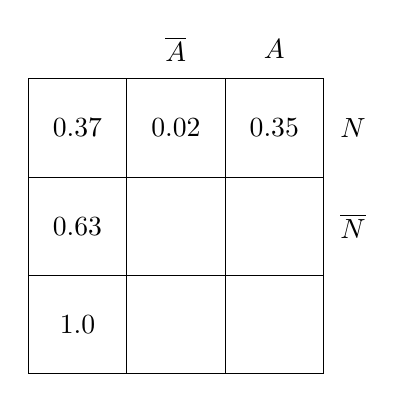
\begin{tikzpicture}[scale=1.25]
\draw (0,0) grid (3,3);
\node at (2.5,3.3) {$A$};
\node at (1.5,3.3) {$\overline{A}$};
\node at (3.3,2.5) {$N$};
\node at (3.3,1.5) {$\overline{N}$};
\node at (2.5,2.5) {$0.35$};
\node at (0.5,2.5) {$0.37$};
\node at (1.5,2.5) {$0.02$};
\node at (0.5,1.5) {$0.63$};
\node at (0.5,0.5) {$1.0$};
\end{tikzpicture}
\end{center}



בהמשך נתון ש:
\[
P(\overline{N}\cap\overline{A})=\frac{P(N\cap A)}{5}=\frac{0.35}{5}=0.07\,,
\]
וניתן להשלים את הטבלה:
\begin{center}
\selectlanguage{english}
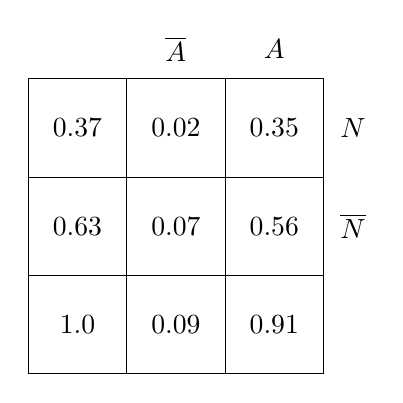
\begin{tikzpicture}[scale=1.25]
\draw (0,0) grid (3,3);
\node at (2.5,3.3) {$A$};
\node at (1.5,3.3) {$\overline{A}$};
\node at (3.3,2.5) {$N$};
\node at (3.3,1.5) {$\overline{N}$};
\node at (2.5,2.5) {$0.35$};
\node at (0.5,2.5) {$0.37$};
\node at (1.5,2.5) {$0.02$};
\node at (0.5,1.5) {$0.63$};
\node at (0.5,0.5) {$1.0$};
\node at (1.5,0.5) {$0.09$};
\node at (2.5,0.5) {$0.91$};
\node at (1.5,1.5) {$0.07$};
\node at (2.5,1.5) {$0.56$};
\end{tikzpicture}
\end{center}

\smallskip

\textbf{סעיף א}

הניסוח "בחרו 
$\ldots$
תלמיד 
$\ldots$
שלא עבר את המבחן. מה ההסתברות
\textbf{שהוא}
נעזר בחבריו?" מכוון להסתברות מותנית:
\[
P(N/\overline{A})=\frac{P(N\cap \overline{A})}{P(\overline{A})}=\frac{0.02}{0.09}=\frac{2}{9}\,.
\]
\textbf{סעיף ב}

הניסוח
\textbf{"ידוע ש"}
מכוון להסתברות מותנית.

עבור יעל ההסתברות המותנית היא:
\[
P(A/N)=\frac{P(A \cap N)}{P(N)}=\frac{0.35}{0.37}=0.9459\,,
\]
ועבור הדס ההסתברות המותנית היא:
\[
P(A/\overline{N})=\frac{P(A\cap \overline{N})}{P(\overline{N})}=\frac{0.56}{0.63}=0.8889\,.
\]
ליעל הסתברות גבוהה יותר לעבור את המבחן.

\smallskip

\textbf{סעיף ג}

שליש (לא שלושה!) של שש הוא שניים. המילה "בדיוק" מכוון לנוסחת
ברנולי הערך
$P(\overline{N}\cap A)=0.56$
נמצא בטבלה ולפי נוסחה ברנולי ההסתברות היא:
\[
{6 \choose 2}(0.56)^2 (1-0.56)^4=0.1763\,.
\]
\textbf{סעיף ד}

הניסוח
"\textbf{לפחות אחת}"
משתי הטענות
\L{I, II}
אומר שמאורע מורכב משני המאורעות
\L{I, II}
או משניהם. בתרשים להלן שני העגולים המייצגים את שני המאורעות
\L{I, II}
כאשר המאורע "לפחות אחת" מיוצג על ידי כל השטח המקווקו:%
\label{p.venn}
\begin{center}
\selectlanguage{english}
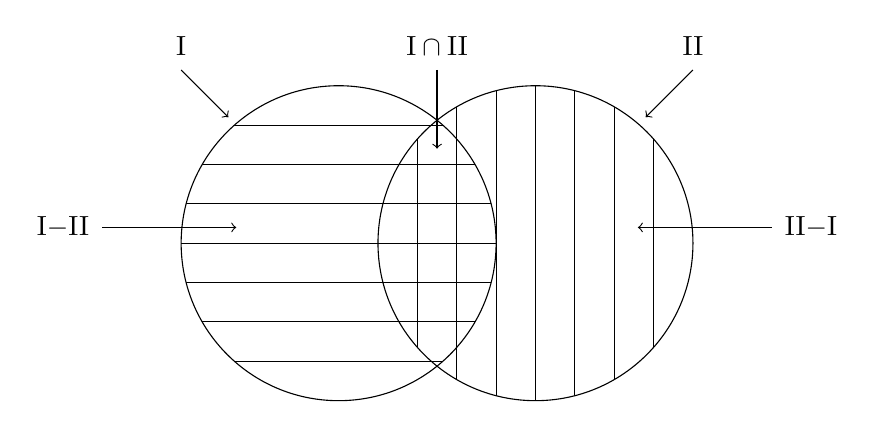
\begin{tikzpicture}
\begin{scope}
\clip[draw] (0,0) circle[radius=2];
\foreach \y in {-1.5,-1,-.5,0,.5,1,1.5}
  \draw (-2,\y) -- (2,\y);
\end{scope}
\begin{scope}
\clip[draw] (2.5,0) circle[radius=2];
\foreach \x in {1,1.5,2,2.5,3,3.5,4}
  \draw (\x,-2) -- (\x,2);
\end{scope}
\node at (-2,2.5) {\textrm{I}};
\node at (4.5,2.5) {\textrm{II}};
\node at (1.25,2.5) {\textrm{I}$\:\cap\:$\textrm{II}};
\node at (-3.5,.2) {\textrm{I$-$II}};
\node at (6,.2) {\textrm{II$-$I}};
\draw[->] (1.25,2.2) -- ++(0,-1);
\draw[->] (-3,.2) -- ++(1.7,0);
\draw[->] (5.5,.2) -- ++(-1.7,0);
\draw[->] (-2,2.2) -- +(.6,-.6);
\draw[->] (4.5,2.2) -- +(-.6,-.6);
\end{tikzpicture}
\end{center}
יש שתי דרכים לחשב את ההסתברות. בדרך הראשונה אנו לוקחים את סכום ההסתברויות של שני המאורעים, ומחסירים את ההסתברות של המאורע המשותף כי ספרנו אותו פעמיים, פעם כחלק מהמאורע
\L{I}
ופעם כחלק מהמאורע
\L{II}:
\[
P(\textrm{I} \cup \textrm{II}) = P(\textrm{I}) + P(\textrm{II}) - P(\textrm{I} \cap \textrm{II})\,.
\]
בדרך השניה אנו סופרים כל חלק מהמאורע השותף בנפרד, כאשר הסימון
\L{I-II}
הוא כל האיברים בקבוצה 
\L{I}
שאינם בקבוצה
\L{II}
ולהיפך:
\[
P(\textrm{I} \cup \textrm{II}) = P(\textrm{I}\:-\:\textrm{II}) + P(\textrm{II}\:-\:\textrm{I}) + P(\textrm{I} \cap \textrm{II})\,.
\]
את ההסתברויות לחישוב ניקח מהטבלה. הדרך הראשונה מופיעה מימין והדרך השניה משמאל:
\begin{center}
\selectlanguage{english}
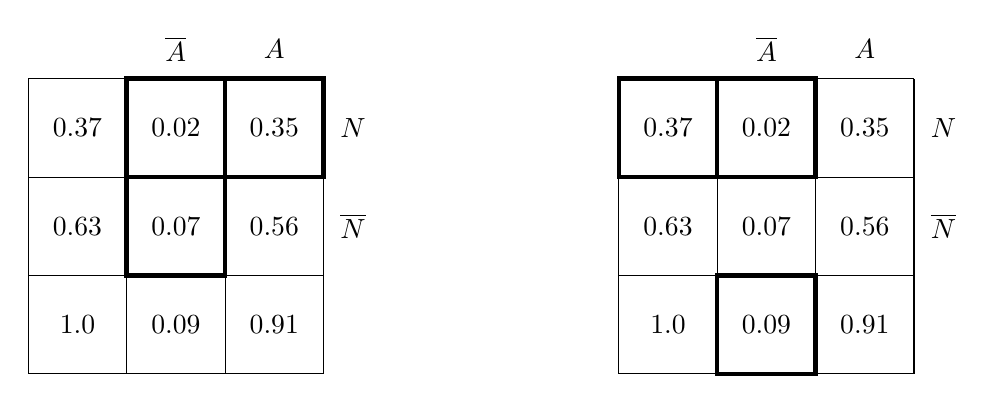
\begin{tikzpicture}[scale=1.25]
\begin{scope}
\draw (0,0) grid (3,3);
\node at (2.5,3.3) {$A$};
\node at (1.5,3.3) {$\overline{A}$};
\node at (3.3,2.5) {$N$};
\node at (3.3,1.5) {$\overline{N}$};
\node at (2.5,2.5) {$0.35$};
\node at (0.5,2.5) {$0.37$};
\node at (1.5,2.5) {$0.02$};
\node at (0.5,1.5) {$0.63$};
\node at (0.5,0.5) {$1.0$};
\node at (1.5,0.5) {$0.09$};
\node at (2.5,0.5) {$0.91$};
\node at (1.5,1.5) {$0.07$};
\node at (2.5,1.5) {$0.56$};
\draw[ultra thick] (2,2) rectangle +(1,1);
\draw[ultra thick] (1,1) rectangle +(1,1);
\draw[ultra thick] (1,2) rectangle +(1,1);
\end{scope}
\begin{scope}[xshift=6cm]
\draw (0,0) grid (3,3);
\node at (2.5,3.3) {$A$};
\node at (1.5,3.3) {$\overline{A}$};
\node at (3.3,2.5) {$N$};
\node at (3.3,1.5) {$\overline{N}$};
\node at (2.5,2.5) {$0.35$};
\node at (0.5,2.5) {$0.37$};
\node at (1.5,2.5) {$0.02$};
\node at (0.5,1.5) {$0.63$};
\node at (0.5,0.5) {$1.0$};
\node at (1.5,0.5) {$0.09$};
\node at (2.5,0.5) {$0.91$};
\node at (1.5,1.5) {$0.07$};
\node at (2.5,1.5) {$0.56$};
\draw[ultra thick] (0,2) rectangle +(1,1);
\draw[ultra thick] (1,0) rectangle +(1,1);
\draw[ultra thick] (1,2) rectangle +(1,1);
\end{scope}
\end{tikzpicture}
\end{center}
בשתי הדרכים מקבלים אותה תוצאה:
\begin{eqn}
P(N\cup\overline{A})&=&P(N) + P(\overline{A}) - P(N\cap\overline{A}) = 0.37+0.09-0.02=0.44\\
P(N\cup\overline{A})&=&P(N-\overline{A}) + P(\overline{A}-N) + P(N\cap\overline{A}) = 0.35+0.07+0.02=0.44\,.
\end{eqn}

%%%%%%%%%%%%%%%%%%%%%%%%%%%%%%%%%%%%%%%%%%%%%%%%%%%%%%%%%%%%%

\newpage

\section{חורף תשע"ח}

\begin{center}
\selectlanguage{english}
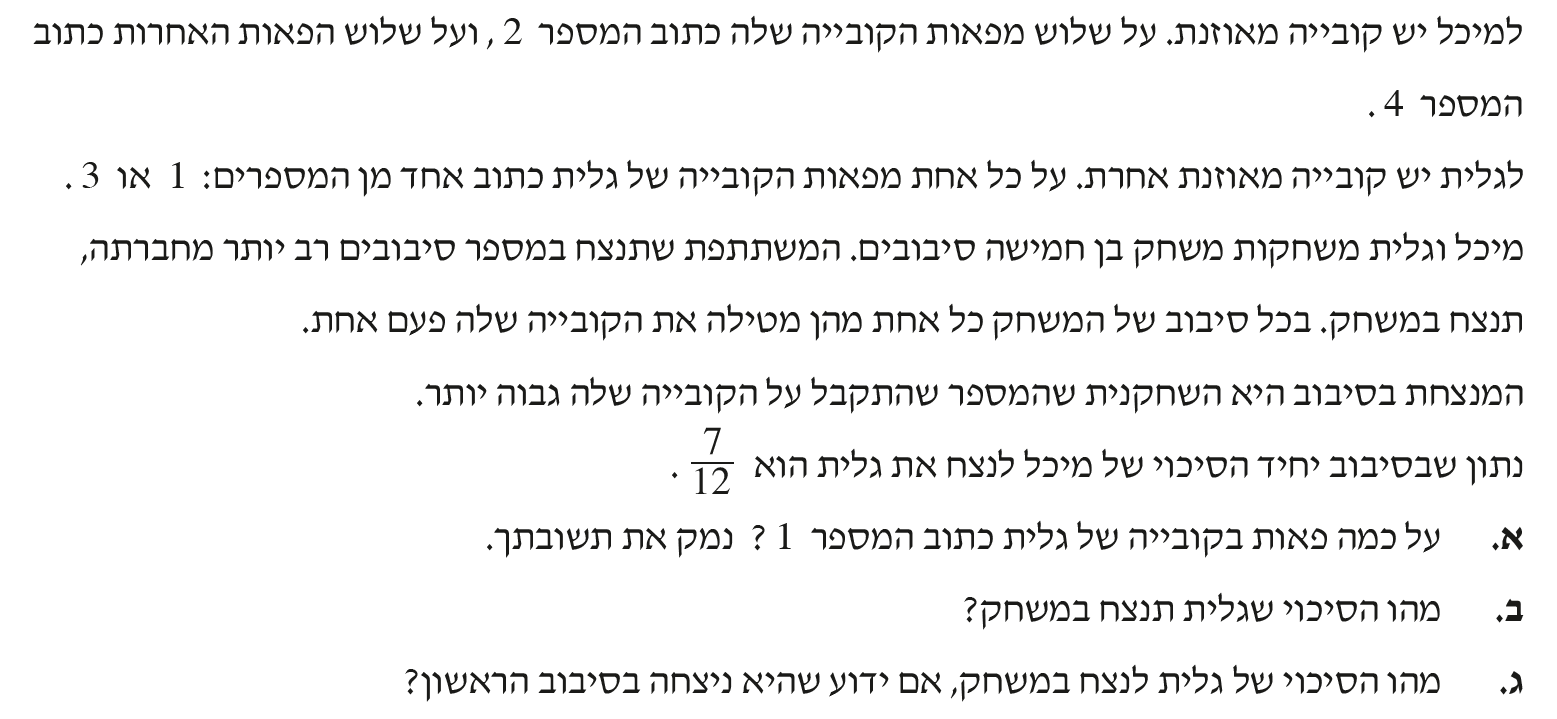
\includegraphics[width=\textwidth]{winter-2018-3}
\end{center}

\textbf{סעיף א}

נסמן ב-%
$n$
את המספר הפאות של הקוביה של גלית שכתוב עליהן
$1$.
מאורע אחד הוא שמיכל תנצח כי היא מטילה 
$4$
בהסתברות
$\frac{3}{6}$
לא משנה מה גלית מטילה. מאורע שני הוא שמיכל תנצח כי היא מטילה 
$2$
בהסתברות
$\frac{3}{6}$
וגלית מטילה
$1$
בהסתברות
$\frac{n}{6}$.
המאורעות זרים זה לזה ולכן:
\begin{eqn}
P(\textrm{\R{מיכל תנצח}}) &=&
\frac{3}{6}\cdot 1 + \frac{3}{6}\cdot \frac{n}{6}=\frac{7}{12}\\
n &=& 1\,.
\end{eqn}
\textbf{סעיף ב}

גלית תנצח אם היא תנצח ב-%
$3,4,5$
סיבובים. נשמתמש בנוסחת ברנולי כדי לקבל את ההסתברות כתלות של ההסתברות של גלית לנצח בסיבוב אחד שהיא המשלים להסתברות שמיכל תנצח
$1-\frac{7}{12}=\frac{5}{12}$:
\[
P(\textrm{\R{גלית תנצח}})={5\choose 3}\left(\frac{5}{12}\right)^3\left(\frac{7}{12}\right)^2+{5\choose 4}\left(\frac{5}{12}\right)^4\left(\frac{7}{12}\right)^1+{5\choose 5}\left(\frac{5}{12}\right)^5\left(\frac{7}{12}\right)^0=0.3466\,.
\]
\textbf{סעיף ג}

הניסוח
\textbf{אם ידוע}
מכוון להסתברות מותנית. נסמן ב-%
$G$
את המאורע שגלית תנצח במשחק וב-%
$R$
את המאורע שהיא תנצח בסיבוב הראשון:
\[
P(G/R) = \frac{P(G \cap R)}{P(R)}\,.
\]
כדי שגלית תנצח במשחק וגם בסיבוב הראשון, היא חייבת לנצח בסיבוב הראשון וגם ב-%
$2$
או
$3$
או
$4$
מהסיבובים הנותרים:
\begin{eqn}
P(G \cap R)&=&\frac{5}{12}\left[{4 \choose 4}\left(\frac{5}{12}\right)^4 \left(\frac{7}{12}\right)^0+
{4 \choose 3}\left(\frac{5}{12}\right)^3 \left(\frac{7}{12}\right)^1+
{4 \choose 2}\left(\frac{5}{12}\right)^2 \left(\frac{7}{12}\right)^2\right]\\
&=&\textstyle\frac{5}{12}\cdot 0.5534\,.
\end{eqn}
כבר חישבנו ש-%
$P(R)=\frac{5}{12}$
ולכן 
$P(G/R)= 0.5534$.
